\usepackage{graphicx}% @author Arian Helberg

\chapter{Softwareprojekt}

\subsection{Vorgehen}
Das Programm zu dieser Arbeit wird mit einem XP-basierten Ansatz erarbeitet.
Hierbei beinhaltet ein \textbf{Release} Funktionen, die insgesamt für eine neue Version des Systems ausreichen;
also ein vollständig funktionsfähiges Programm liefern.
\textbf{User Stories} sind innerhalb der Iterationen umzusetzende Teilaufgaben und deren Aufwandseinschätzung gibt
Auskunft über den Entwicklungsaufwand einer Umsetzung.\\~\\
Umsetzung des Softwareprojektes in Iterationen mit folgenden Phasen:
\begin{itemize}
    \item Planung:
    \begin{itemize}
        \item Release-Planung:\\"`\textit{Welche Features werden in diesem Release umgesetzt?}"',\\User Stories,
        Aufwandsschätzung, Anforderungsmanagement
        \item Iterationsplanung:\\Umwandlung der User Stories in kleine Arbeitsschritte,\\Festlegen der Dauer einer
        Implementierung
    \end{itemize}
    \item Entwurf: Architektur, Klassendiagramme, Schnittstellen
    \item Testing: (Automatisierte) Modul- und Regressionstests
    \item Programmierung: Umsetzung der Features, Implementierung, Modularisierung
\end{itemize}
\begin{figure}[H]
    \centering
    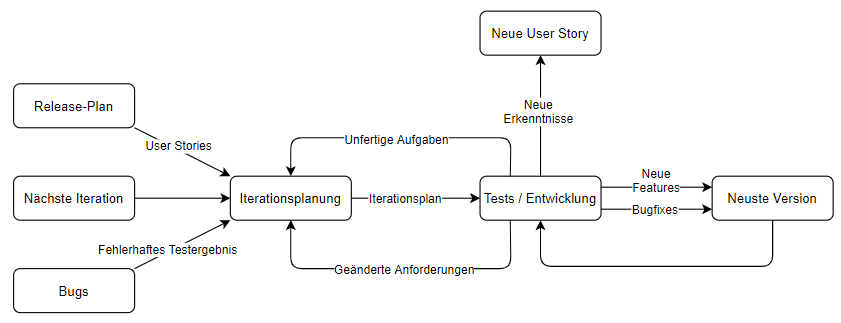
\includegraphics[width=15cm]{../../images/extreme_programming.PNG}
    \caption{Ablaufdiagramm}
\end{figure}